\section{Desarrollo de subsistemas}

Para este proyecto hemos desarrollado dos subsistemas analógicos propios, sobre dos PCB distintas, una de alimentación y un amplificador de audio. Además, hemos utilizado tres subsistemas ya existentes para la recepción de audio, la reproducción de música en MP3 y la lectura de información NFC de un dispositivo móvil.

\subsection{La placa}
Para este proyecto se ha utilizado la placa \texttt{STM32F769NI-DISCO}, que es una placa de desarrollo comercializada por STM. Dispone de un procesador ARM Cortex M7, que puede funcionar a una frecuencia de hasta 216 MHz. 

Dispone de pines dispuestos de una forma adecuada para ser compatible con Arduino Uno.

Entre los periféricos presentes en la placa, los más importantes que utilizamos son:
\begin{itemize}
    \item \textbf{La pantalla:} Dispone de una pantalla LCD táctil de 4.3 pulgadas, accesible a través del periférico DSI, con una resolución de 800 x 480 píxeles, con una profundidad del  color de 16 bits, lo que resulta en un total de $2^{16}$ colores posibles de representar. En concreto, se asignan 5 bits para las componentes roja y azul, siendo los 6 restantes para la verde, que es la más importante.
    \item \textbf{La DMA2:} La pantalla restringe el uso de las DMA, siendo la 2 la única opción posible, puesto que es la única que tiene la opción de \textit{Memory-To-Memory}. Cualquier canal y flujo (\textit{Channel} y \textit{Stream}) son de libre elección.
    \item \textbf{Los ADCs:} La placa dispone tres ADCs, que funcionan a una frecuencia de 48 kHz, de los cuales nuestro proyecto utiliza dos: el ADC1 se utiliza para medir el consumo, y el ADC3 se utiliza como pin de entrada para el audio. 
    \item \textbf{El DAC:} La placa dispone de un DAC de 2 canales. En la documentación de la placa no se anuncia esta capacidad, únicamente se puede encontrar el la documentación del microcontrolador. El DAC también funciona a 48kHz, y se sincroniza con el ADC, como se explica en \autoref{para:temporizacion}.
    \item \textbf{El I2C:} Utilizamos un I2C para la comunicación con el módulo del NFC.
    \item \textbf{La SD:} Dispone de un puerto para introducir una tarjeta SD, a través del periférico SDMMC.
\end{itemize} 

\subsubsection{Algunas consideraciones}
En algunos proyectos, hemos intentado utilizar la sentencia \texttt{printf}, pero a priori parecía una tarea imposible. Revisando la documentación, constatamos que el pin \texttt{SW0} está desconectado en la configuración por defecto. Para que funcione dicha función, hay que soldar \texttt{R92}, que conecta \texttt{SW0} con el pin adecuado. Esta resistencia funciona como un jumper, ya que el valor anunciado por el fabricante es de 0 $\Omega$. Tras sujetar un cable de forma manual, conseguimos visualizar la salida de la \texttt{UART} desde el panel del debugger.
\subsection{Subsistema de alimentación}

El subsistema de alimentación es el encargado de permitir que el sistema se alimente a través de baterías. También permite cargar la batería e incluso ambas acciones simultáneamente.

Como batería hemos decidido utilizar una batería de ion de litio 18650, un modelo bastante estándar en las aplicaciones integradas.  Concretamente, hemos decidido utilizar el modelo \texttt{INR18650-29E} de Samsung, que tiene una tensión nominal de 3.7\ V y una capacidad de 2900\ mAh.

Sin embargo, este tipo de baterías tienen unos requisitos de carga muy estrictos. Contando con que la batería parte de un estado correcto (no por debajo del límite de tensión segura), se debe cargar primero con un método de corriente constante hasta alcanzar una tensión cercana a la máxima y después cambiar a un método de tensión constante hasta finalizar la carga \cite{BU409ChargingLithiumion}. Un ejemplo de ciclo de carga se puede ver en la \autoref{fig:2-1-cicloCarga}

\begin{figure}[h]
    \centering
    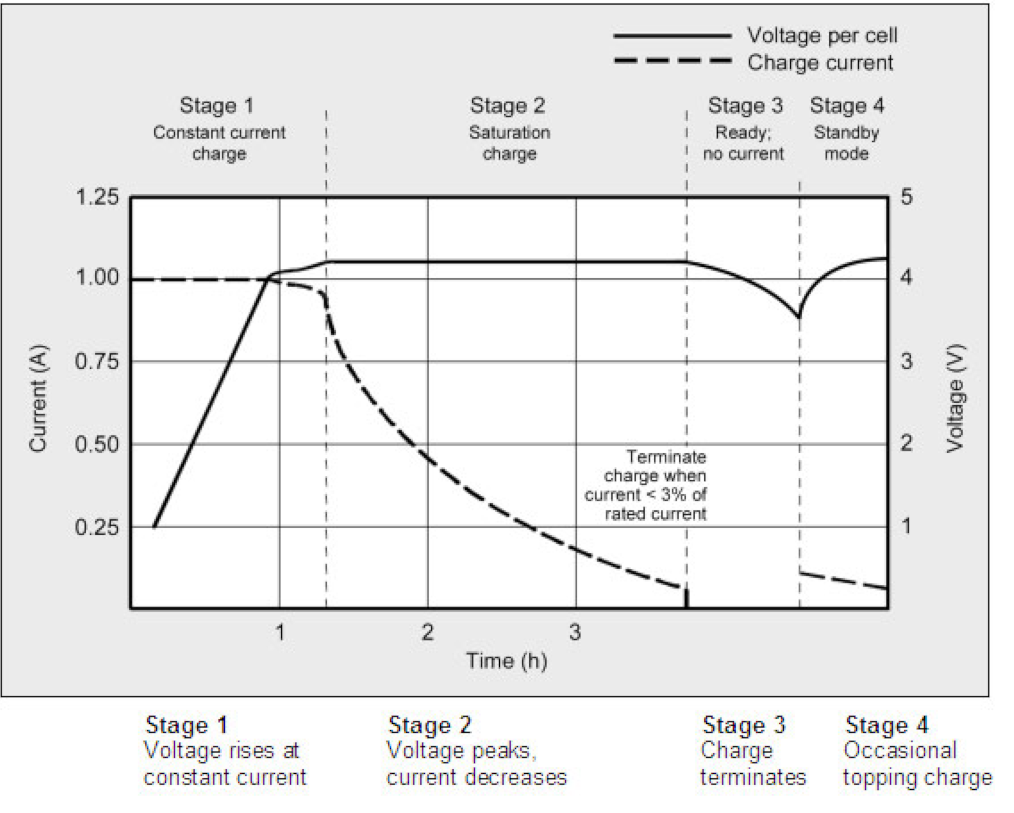
\includegraphics[width=0.5\textwidth]{images/2/2-1/cargaBateria.png}
    \caption{Ciclo de carga de una batería de ión de litio}
    \label{fig:2-1-cicloCarga}
\end{figure}

Si no se respeta el ciclo de carga de estas baterías, se tiene una alta probabilidad de que falle de forma violenta, siendo incluso un peligro de incendio. 

\subsubsection{Circuito de carga}

Para facilitarnos la tarea de respetar este ciclo hemos utilizado una solución integrada de Texas Instruments, el \texttt{BQ25606}, un cargador de una celda de litio que soporta hasta 3 amperios de corriente. \cite{BQ25606DataSheet}

Gracias a este circuito integrado y bastantes componentes externos, podemos diseñar un circuito que, a partir de una tensión de entrada entre 5 y 12 voltios y utilizando un convertidor reductor, carga la batería adecuadamente y de forma segura. 

La entrada al circuito puede ser a través de un conector \textit{Jack} de alimentación o un conector \textit{Micro USB}. Además, si se utiliza el segundo conector, el integrado se encarga de negociar el protocolo de carga rápida con la fuente de alimentación para incrementar la corriente de entrada y mejorar la potencia de carga. 

Además, si el circuito está conectado a la alimentación y la fuente tiene suficiente capacidad, la corriente de salida se obtiene de la entrada en lugar de la batería, gracias a la tecnología PowerPath de TI. Esta tecnología además permite balancear las tres corrientes, por lo que si el sistema requiriera de más corriente de la que la fuente de alimentación pudiera proveer, se obtendría también de la batería realizando un esfuerzo coordinado entre la fuente y la batería. Si por el contrario la fuente puede ofrecer más corriente de la que se está solicitando en la salida, se utiliza este excedente para cargar la batería.

Este circuito cuenta además con dos indicadores LED que informan sobre si la fuente de alimentación está conectada y las tensiones son correctas (verde en nuestro circuito) y si se está cargando la batería o hay algún fallo (roja en nuestro circuito). La segunda luz se mantiene encendida mientras se está cargando, se apaga cuando se ha finalizado la carga y parpadea a 1 Hz de frecuencia si hay algún error.

Para ofrecer todas estas características, el circuito integrado consta de una máquina de estados finitos y múltiples comparadores de error. Con esta inteligencia conmuta tres transistores para conectar la batería y para gestionar el convertidor conmutado síncrono que se construye. Se puede ver un diagrama de bloques resumido del circuito (obtenido de la hoja de catálogo) en la \autoref{fig:2-1-bloquesInternosBQ25606}

\begin{figure}[h]
    \centering
    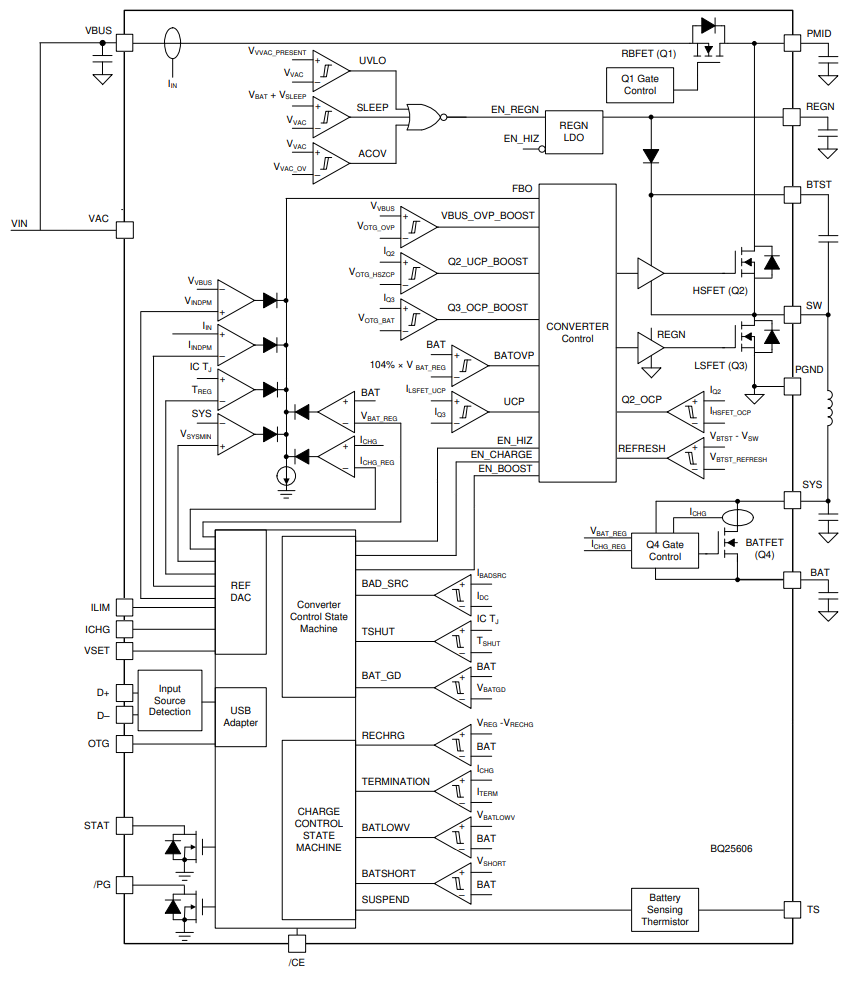
\includegraphics[width=0.5\textwidth]{images/2/2-1/BQ25606Bloques.png}
    \caption{Diagrama de bloques interno del BQ25606}
    \label{fig:2-1-bloquesInternosBQ25606}
\end{figure}

Este circuito ofrece a su salida una tensión aproximadamente igual a la de la batería durante el funcionamiento normal, por lo que está alrededor de los 3.7 V. Sin embargo, si la tensión de la batería cae por debajo de 3.5 V, el circuito se encarga de ofrecer dicha tensión a la salida, por lo que nunca bajará de dicho valor (mientras la batería puede ofrecer corriente y no esté descargada).

El circuito integrado ofrece también la posibilidad de utilizar una batería con sensor de temperatura integrado, pero no vamos a utilizarlo debido al incremento en coste de la misma.

En la hoja de catálogo del integrado se ofrece información sobre el proceso de diseño de un circuito alrededor de dicho integrado. Además, se tiene una nota de aplicación sobre el diseño de circuitos alrededor de este integrado \cite{texasinstrumentsDesigningStandaloneSingle}:

\begin{itemize}
    \item Inductancia de 2.2 $\mu$ F para reducir el rizado de corriente.
    \item Pin \texttt{VSET} flotante para tensión de carga máxima de 4.208 V.
    \item Divisor de tensión de dos resistencias de 10 $k\Omega$ en \texttt{TS} para no utilizar divisor de tensión.
    \item Resistencia de 165 $\Omega$ en \texttt{ILIM} para limitar la corriente de entrada cuando no se negocia carga rápida a 3 A (normalmente se utiliza mucho menos).
    \item Resistencia de 487 $\Omega$ en \texttt{ICHG} para limitar la corriente de carga máxima a 1.4 A como se indica en las especificaciones de la batería.
    \item El resto de componentes se toman de la Figura 10-1 de la hoja de catálogo
\end{itemize}

Por tanto, esta parte del circuito queda como se puede ver en la \autoref{fig:2-1-circuito-carga-final}.

\begin{figure}[h]
    \centering
    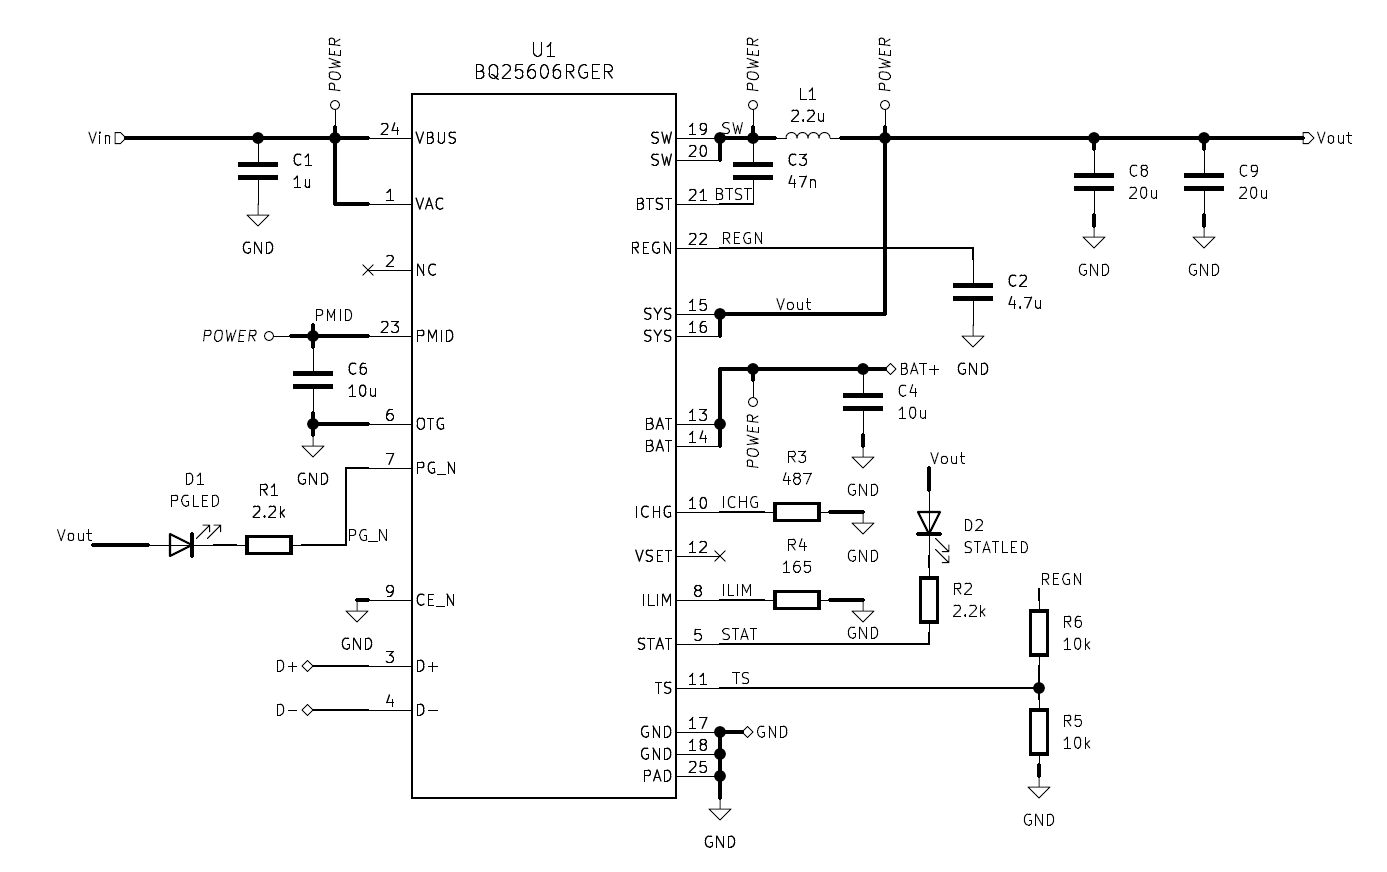
\includegraphics[width=\textwidth]{images/2/2-1/circuitoCarga.png}
    \caption{Subcircuito de carga de batería}
    \label{fig:2-1-circuito-carga-final}
\end{figure}

\subsubsection{Convertidor elevador}\label{subsubsec:convertidor_elevador}

La placa que utilizamos especifica una tensión de entrada de 7 V a 12 V si se utiliza el pin $V_{in}$ inferior. Preferimos utilizar este método ya que la entrada de 5 V no tiene protección y se puede dañar la placa si no se realiza todo el proceso adecuadamente.

Experimentalmente hemos notado que la placa utiliza la misma corriente de entrada para cualquier valor de tensión, por lo que seguramente utilice un convertidor de tensión lineal internamente para generar las tensiones. Por tanto, hemos preferido tomar el valor más pequeño de las tensiones de entrada para reducir la pérdida de potencia.

La tensión de salida del circuito de carga oscila entre los 3.5 V y los 4.2 V, por lo que hemos diseñado un convertidor conmutado elevador o \textit{Boost Converter} para obtener dicha tensión a partir de la salida del cargador.

Un circuito convertidor elevador está compuesto básicamente por una bobina, un transistor y un controlador PWM.\ Como controlador PWM hemos utilizado otra solución integrada de Texas Instruments debido a la alta precisión que nos permite tener, ya que un fallo en este circuito podría dañar seriamente al resto del sistema. 

El circuito integrado elegido es el LM51561H. Este circuito es un controlador de convertidores conmutados de tipo \textit{Boost, SEPIC} y \textit{Flyback} con gran rango de tensiones y muy elevada protección. \cite{LM51561HDataSheete}

Además, indica específicamente que está pensado para aplicaciones de batería gracias a su baja tensión de entrada necesaria para funcionar. Al contrario que el circuito del cargador, este integrado no incluye los transistores internos por lo que se tienen que añadir externamente. 

Este integrado consta básicamente de comparadores de error respecto a tensiones de referencia y un generador de señales triangulares para la generación de PWM. Cuenta además con la posibilidad de compensar el circuito para evitar su inestabilidad. La versión LM51561H es igual que la LM5156H solo que con protección en modo \textit{Hiccup}. En este modo de protección, si se detecta una sobrecarga, se desactiva el convertidor y se comienza una espera. Al finalizar la espera, se trata de volver a arrancar la conversión. Si la condición de sobrecarga sigue presente, se vuelve a dormir y repetir el ciclo. Esto permite una mucho menor potencia media en condición de sobrecarga en comparación a la protección por corriente media, pico o valle. \cite{hariImprovePowerConverter}

Se puede ver un diagrama de bloques resumido en la \autoref{fig:2-1-LM51561H-bloques}.


\begin{figure}[h]
    \centering
    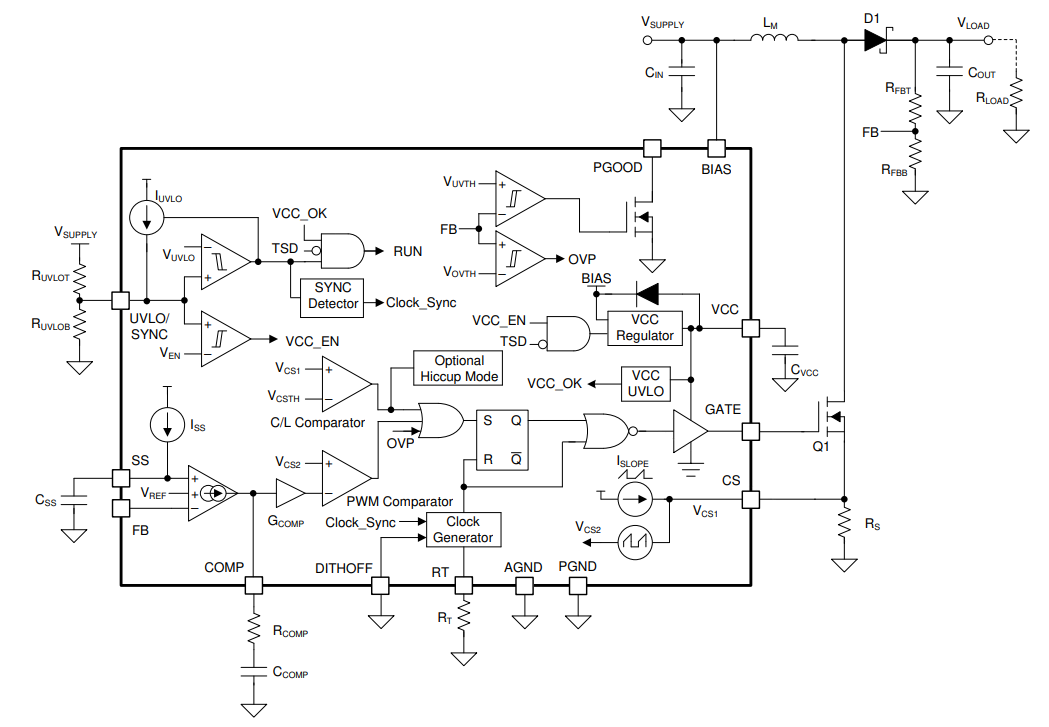
\includegraphics[width=0.5\textwidth]{images/2/2-1/LM51561HBloques.png}
    \caption{Diagrama de bloques interno del LM51561H}
    \label{fig:2-1-LM51561H-bloques}
\end{figure}

Algunas de las características destacables de nuestro circuito son:
\begin{enumerate}
    \item Protección contra infravoltaje (\textit{Undervoltage Lockout}). Se comprueba que el pin \texttt{UVLO} tenga una tensión superior a 0.55 V para comenzar la configuración interna y superior a 1.5 V para comenzar a conmutar.
    \item Frecuencia elevada de conmutación para evitar interferencias en las bandas de AM y reducir las pérdidas de conmutación.
    \item Salida de 7 V muy estable y con poca dependencia de la corriente de salida
\end{enumerate}

Para el diseño de este circuito, el fabricante recomienda el uso de la herramienta WEBENCH Power Designer\footnote{\url{https://www.ti.com/tool/download/SNVC224}}, que permite reducir la complejidad del diseño realizando los cálculos necesarios para los parámetros deseados y la compensación de la función de transferencia del circuito. 

Utilizando dicha herramienta, generamos el circuito que hemos utilizado con los siguientes parámetros: 
\begin{enumerate}
    \item $V_{in, \min} = 3.5\ V$
    \item $V_{in, \max} = 4.2\ V$
    \item $V_{out} = 7.0\ V$
    \item $I_{out} = 1.0\ A$
\end{enumerate}

Una vez introducidos los parámetros, el software genera el circuito con los componentes recomendados, permitiendo sustituirlos por equivalentes y generando las gráficas de funcionamiento aproximado. Se puede encontrar el reporte generado en el \autoref{anexo:webench-report}

Con el resultado de dicho software, se construye un circuito como el de la \autoref{fig:2-1-circuito-boost-final}.

\begin{figure}[h]
    \centering
    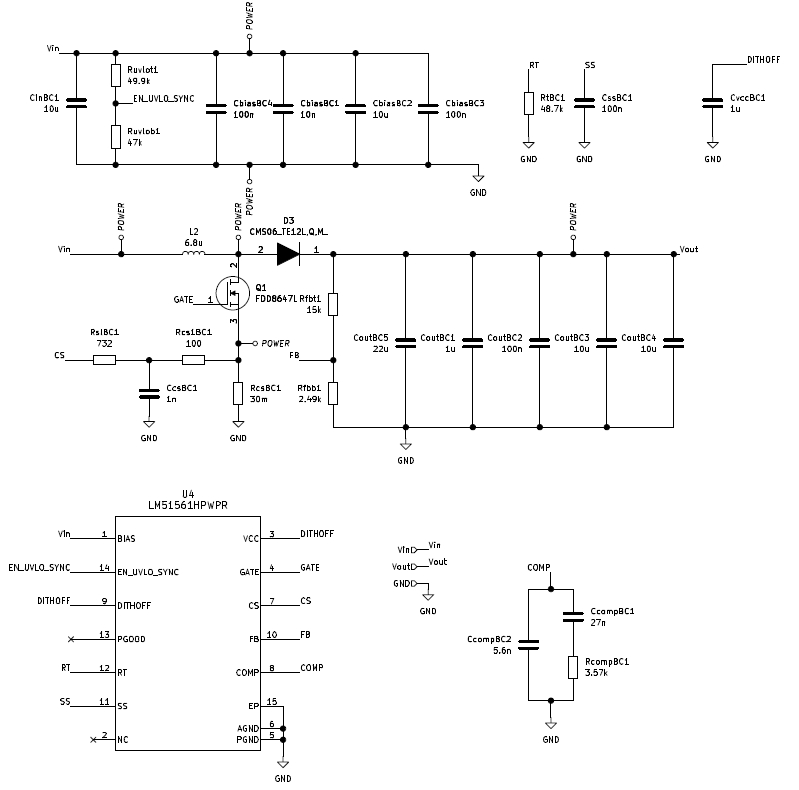
\includegraphics[width=0.5\textwidth]{images/2/2-1/circuitoElevador.png}
    \caption{Circuito del convertidor elevador}
    \label{fig:2-1-circuito-boost-final}
\end{figure}

\subsubsection{Medidor de consumo}
\label{subsubsec:medidor-consumo-analog}

Otra parte importante de este circuito es el medidor de consumo integrado. Para ello, primero pensamos en construir un amplificador de instrumentación, que se puede adquirir ya implementado en un mismo paquete o realizar con dos amplificadores operacionales. Sin embargo, durante la búsqueda de modelo de amplificador operacional encontramos un modelo que se ofrece como especializado en medición de corriente en el nivel bajo (\textit{Low-side current switching}) por lo que decidimos quedarnos con él.

Dicho integrado es el OPA187ID, un amplificador operacional de precisión con aproximadamente cero tensión de offset ($10\ \mu V$, $0.001\mu V/^\circ\! C$). \cite{OPA187DataSheet}

Dicho amplificador operacional recomienda montar una configuración de amplificador diferencial con una resistencia \textit{shunt} de muy baja impedancia y configurar la ganancia deseada mediante las resistencias de realimentación.

Como resistencia de medida hemos elegido un valor bajo, de $10\ m\Omega$ y que soporta 1 W de potencia. Para simplificar los cálculos, hemos decidido asignar el rango de entrada de un ADC de nuestra placa ($[0, 3.3]\ V$) a un rango de $[0, 3]\ A$. Por ello, la ganancia es:

\[
    G = \frac{3.3 - 0}{3 - 0} = 1.1 V/A  
\]

Para conseguir dicha ganancia es tan sencillo como utilizar resistencias con un cociente de 110, por lo que elegimos valores de $1\ k\Omega$ y $110\ k\Omega$ en el circuito, por lo que obtenemos el circuito de la \autoref{fig:2-1-medidor-consumo}.

\begin{figure}[h]
    \centering
    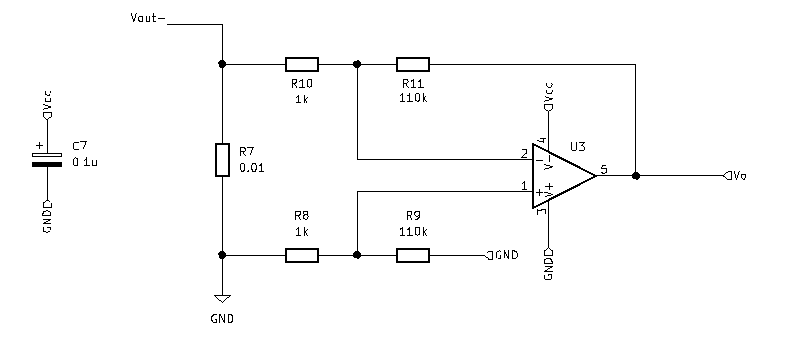
\includegraphics[width=0.5\textwidth]{images/2/2-1/circuitoConsumo.png}
    \caption{Circuito medidor de consumo}
    \label{fig:2-1-medidor-consumo}
\end{figure}

\subsubsection{Diseño de PCB}

Los tres circuitos se han integrado en una sola PCB, permitiendo una mucho mejor integración y uso mucho más sencillo. Se ha integrado un zócalo para insertar la batería sobre la placa y evitar la posibilidad de una mala conexión. Además, se han incluido los conectores de entrada de potencia previamente mencionados, tanto el Jack de alimentación como el conector micro-USB. Por otro lado, la salida del sistema se realiza a través de unos terminales de tornillo que incluyen la tensión de alimentación positiva, negativa y la medida de consumo.

Sin embargo, por un problema durante el ensamble de la placa, se destruyeron los pads del conector micro-USB, por lo el conector no funciona correctamente. Sin embargo, el sistema funciona perfectamente a través del Jack de alimentación.

La alta complejidad de los circuitos integrados hace que sus empaquetados sean muy pequeños, por lo que la soldadura se ha tenido que realizar mediante horno y con stencil. Sin embargo, esto nos ha permitido colocar los componentes muy próximos entre sí, reduciendo el ruido electromagnético generado y las componentes parásitas del circuito. Concretamente, el circuito integrado de carga es de empaquetado \texttt{VQFN24} con un tamaño de $4x4\ mm$ y el integrado del conversor es \texttt{HTSSOP14} con un tamaño de $5x4.4\ mm$.

Además, el pequeño tamaño de estos circuitos reduce significativamente su capacidad de disipación térmica. Por ello, ambos incluyen un pad en su parte inferior que debe ser soldado a un pad que además incluya muchas vias térmicas a la capa inferior, en la que debe haber un plano de tierra grande para disipar el calor que se genere. Por ello y para ofrecer un camino de retorno a las altas corrientes que recorren este circuito, la capa inferior se dedica casi exclusivamente a la masa del circuito. 

Ambos circuitos integrados ofrecen indicaciones sobre la disposición de los componentes que se han seguido rigurosamente. Por ejemplo, se recomienda mantener los bucles de conmutación lo más pequeños posibles o mantener separadas las tierras digital y analógica, juntandolas únicamente en un punto. 

Ciertas zonas del circuito han tenido que ser diseñadas mediante polígonos especiales al no poderse realizar la conexión mediante pistas normales o necesitar zonas especialmente grandes para caminos de mucha corriente.

Se puede ver el resultado final del circuito de alimentación en la \autoref{fig:2-1-circuito-alimentacion}.

\begin{figure}[h]
    \centering
    \includegraphics[width=0.5\textwidth]{images/2/2-1/circuitoAlimentación.jpg}
    \caption{Circuito de alimentación}
    \label{fig:2-1-circuito-alimentacion}
\end{figure}

Se tiene un esquema completo del circuito en el \autoref{anexo:circuito-alimentacion}
\clearpage
\subsection{Subsistema de audio}

El subsistema analógico de audio tiene tres funciones principales:
\begin{enumerate}
    \item Multiplexar las dos entradas de audio (MP3 y Radio) a un ADC del microcontrolador
    \item Multiplexar la salida proveniente del DAC a una de las dos salidas de audio (Altavoces o auriculares)
    \item Amplificar la salida de audio seleccionada
\end{enumerate}

\subsubsection{Divisor de rail}
Este sistema se alimenta directamente desde el módulo de alimentación explicado en el apartado anterior. Por ello, cuenta con una entrada unipolar de 7 voltios. Sin embargo, los circuitos de audio necesitan alimentación bipolar para funcionar. Por ello, hemos decidido implementar un circuito divisor de rail, que genera una tensión intermedia que se utilizará como nueva referencia del circuito, obteniendo una alimentación virtual de $\pm$3.5 V.

El circuito utilizado es un divisor de tensión de precisión implementado mediante el amplificador operacional \texttt{OP07}. Este amplificador operacional tiene muy bajo error estático y además cuenta con dos terminales para el ajuste del offset mediante un potenciómetro, por lo que es ideal para nuestra aplicación.

Sin embargo, los amplificadores operacionales permiten muy poca corriente a través de su terminal de salida, por lo que se necesita un circuito que permita incrementar la corriente de salida o entrada de dicho circuito sin afectar demasiado a la salida. Para ello, se utiliza una topología \textit{Push-Pull} en la que se utilizan dos pares de Darlington, es decir, cuatro transistores, para incrementar la capacidad de corriente del circuito. 

Al introducirlos dentro del lazo de realimentación, se elimina el efecto de las tensiones de base y se elimina el ruido que pudieran introducir, pero a cambio introducen la posibilidad de inestabilizar el circuito. Teniendo esta posibilidad en cuenta, incluimos la posibilidad de soldar un condensador entre el terminal de salida del amplificador y la alimentación negativa del circuito, para introducir un polo que compense la estabilidad. Sin embargo, hemos acabado no necesitando utilizarlo. 

Por tanto, el circuito generador de tierra virtual o divisor de rail queda como se puede ver en la \autoref{fig:2-2-tierra-virtual}.

\begin{figure}[h]
    \centering
    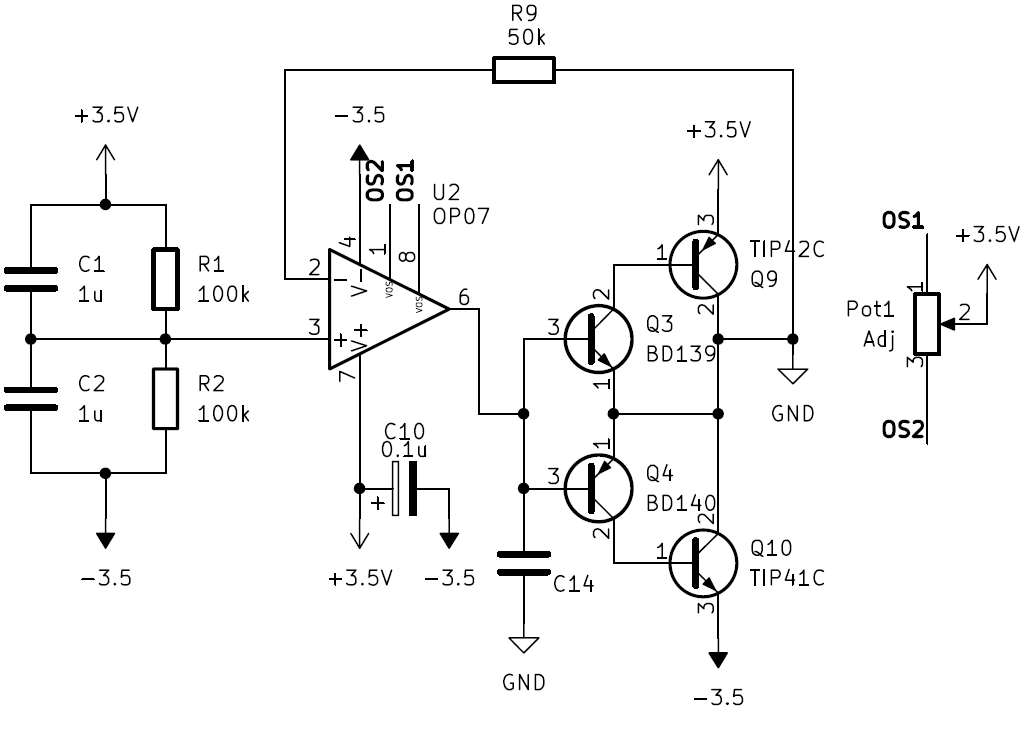
\includegraphics[width=0.5\textwidth]{images/2/2-2/circuitoDivisorRail.png}
    \caption{Circuito divisor de raíl}
    \label{fig:2-2-tierra-virtual}
\end{figure}

\subsubsection{Habilitación del circuito}

Para eliminar el consumo parásito del circuito cuando el sistema entre en el modo bajo consumo, se ha implementado un subcircuito de habilitación el cual permite encender o apagar el resto de subsistema (aunque finalmente el consumo parásito es muy pequeño).

Dicho circuito consiste en un transistor MOSFET de canal N en la alimentación, que permite cortar o dejar pasar la alimentación. Además, la baja impedancia de conducción del transistor permite que no haya casi pérdidas de potencia en el transistor. Sin embargo, ya que para cortar el transistor se necesita polarizar la puerta con una tensión próxima a 7 voltios y soportar las corrientes de los transitorios de conmutación, se utiliza otro transistor con una resistencia de \textit{pull-up} para adaptar los niveles los GPIO y reducir la corriente necesaria. Esto tiene el efecto añadido de invertir la polaridad de la habilitación que junto a la inversión del canal N se anulan, provocando que un nivel alto en el GPIO habilite el circuito. 

Por tanto, el circuito final es el que se ve en la \autoref{fig:2-2-circuito-habilitacion}.

\begin{figure}[h]
    \centering
    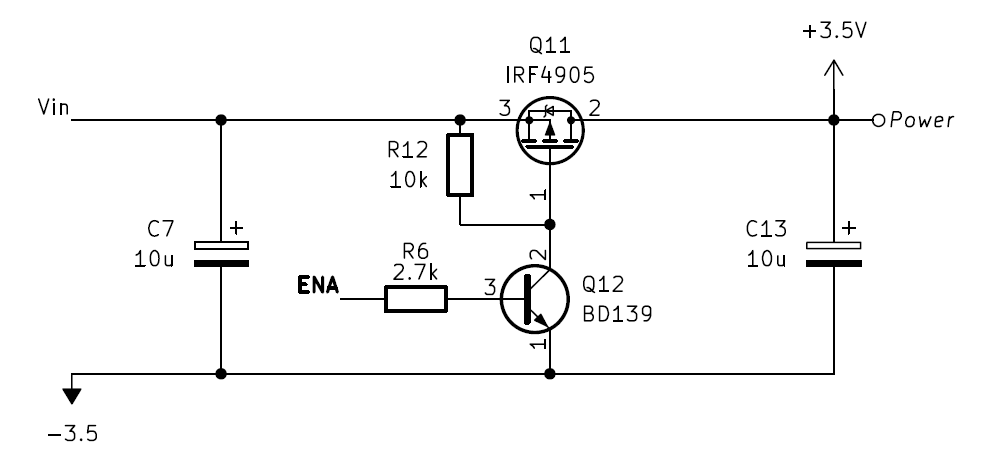
\includegraphics[width=0.5\textwidth]{images/2/2-2/circuitoHabilitacion.png}
    \caption{Circuito de habilitación}
    \label{fig:2-2-circuito-habilitacion}
\end{figure}

\subsubsection{Multiplexación de audio}

Para la multiplexación de audio se va a utilizar un multiplexor integrado. Inicialmente tratamos de diseñar un circuito que multiplexara los caminos de audio mediante componentes discretos, encontrando la estructura de la Puerta de Transmisión \cite{TransmissionGate}, como la que se puede ver en la \autoref{fig:2-2-puerta-transmision}

Sin embargo, todas las estructuras discretas que encontramos necesitan una familia de transistores de efecto de campo en los que el canal no está unido internamente al sustrato, permitiendo cargar la capacidad puerta-canal sin afectar a la tensión del camino drenador-surtidor. 

El principal problema de estos transistores es su elevado precio y muy poca variedad, siendo casi imposible encotrarlos. Además, generalmente se utilizan en aplicaciones de alta potencia por lo que su rendimiento para aplicaciones de baja señal suele ser bastante pobre.

\begin{figure}[h]
    \centering
    \includegraphics[width=0.3\textwidth]{images/2/2-2/puertaTransmisión.png}
    \caption{Puerta de transmisión con transistores con canal desconectado}
    \label{fig:2-2-puerta-transmision}
\end{figure}

Finalmente, descartamos la idea de utilizar componentes discretos y utilizamos una solución integrada. Por tanto, utilizamos el multiplexor analógico \texttt{CD4053BC}. \cite{CD4053BDataSheet}

Este multiplexor cuenta con tres canales en configuración \texttt{SPDT}, por lo que cada canal tiene un terminal en un extremo y dos en el otro. Este multiplexor cuenta con la ventaja de ser bidireccional, cosa de la que muchos otros carecen y es fundamental para nuestra funciononalidad.

Este multiplexor se utiliza para conectar las dos entradas de audio, que provienen de conectores Jack de audio de 3.5 mm a un GPIO que se conecta internamente a un ADC de la placa y para conectar otro GPIO que se conecta internamente a un DAC a las entradas de los dos caminos de amplificación de audio. 

\subsubsection{Cambiador de nivel lógico}

Un error que cometimos es no tener en cuenta la tensión de habilitación necesaria para conmutar un canal del multiplexor, por lo que los 3.3V de salida de un GPIO no son suficientes para cambiar el canal del multiplexor. Esto provoca que se esté siempre seleccionado el canal correspondiente al nivel bajo.

Para solucionar esto, hemos construido un circuito cambiador de nivel lógico que adapta los 3.3 V de la placa a los 7 V necesarios para conmutar el multiplexor (realmente el mínimo es aproximadamente 5V).

La solución que hemos pensado consiste en un inversor lógico TTL, que consiste en un transistor bipolar NPN con una resistencia de \textit{Pull-up}. La única desventaja es la inversión de nivel, pero se corrige fácilmente en el software.

Se puede ver el diagrama de nuestra solución en la \autoref{fig:2-2-cambiador-nivel}, en la que se muestra un cambiador. Hemos soldado dos de ellos en una placa de prototipado, que se puede ver en la \autoref{fig:2-2-foto-cambiador}.

\begin{figure}[h]
    \centering
    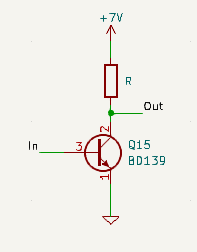
\includegraphics[width=0.5\textwidth]{images/2/2-2/circuitoCambiadorNivel.png}
    \caption{Circuito cambiador de niveles}
    \label{fig:label}
\end{figure}

\begin{figure}[h]
    \centering
    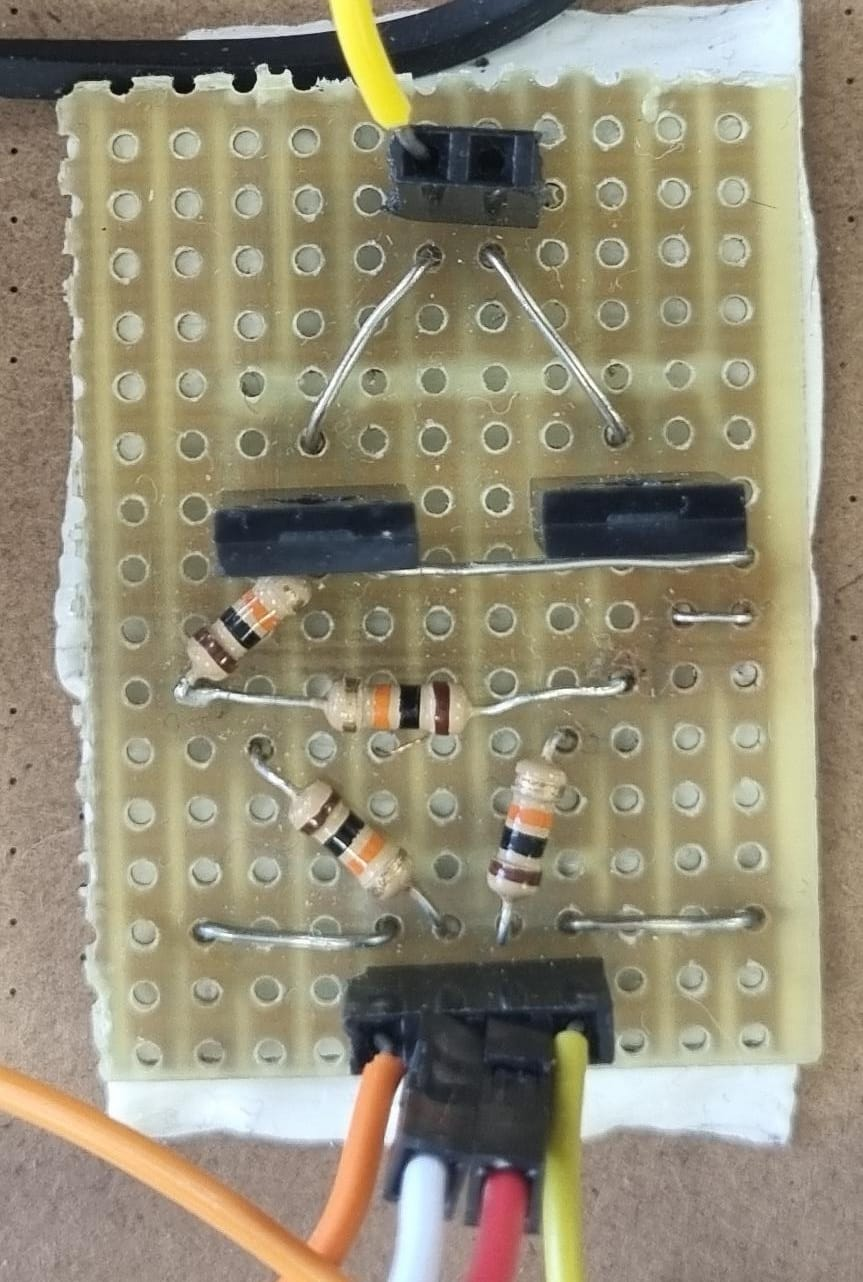
\includegraphics[width=0.25\textwidth]{images/2/2-2/cambiadorNivel.jpg}
    \caption{Foto del circuito cambiador de nivel}
    \label{fig:2-2-foto-cambiador}
\end{figure}
\subsubsection{Amplificador de audio para los auriculares}

La salida del DAC de la placa es una señal entre 0 y 3.3 V con 12 bits de resolución. Por tanto, el audio que se genere tiene una componente continua que se debe eliminar. 

Para eliminar esta componente continua hemos implementado una configuración de filtro paso alto mediante un filtrado pasivo y un seguidor de tensión realizado con un amplificador operacional. En el camino de realimentación del amplificador operacional se coloca una resistencia para anular la tensión de error de \textit{offset} del amplificador operacional.

También se añade la misma estructura de transistores que en el circuito generador de tierra virtual, que ahora al estar también dentro del lazo de realimentación cuentan con la ventaja de que se anula la distorsión de cruce. 

Los valores elegidos para los componentes del filtro son una resistencia de $100\ k\Omega$ y un condensador de $100\ nF$. Con ello, conseguimos una frecuencia de corte de:

\[
    f_c = \frac{1}{2\pi RC} \approx 16\ Hz    
\]

Elegimos este valor ya la banda de audición humana máxima es de $20$ Hz a $20$ kHz.

Se puede ver un diagrama de la solución que montamos en la \autoref{fig:2-2-amp-cascos}.

\begin{figure}[h]
    \centering
    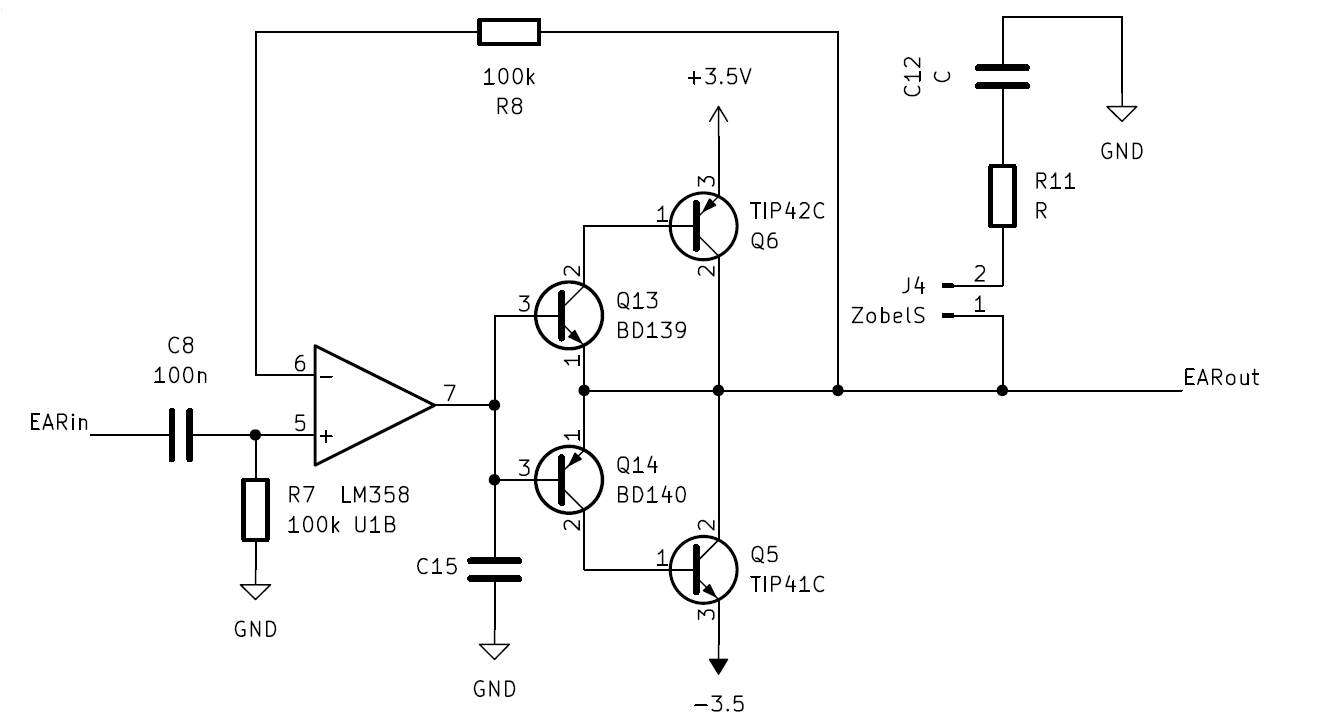
\includegraphics[width=0.7\textwidth]{images/2/2-2/circuitoAmplificadorCascos.png}
    \caption{Circuito amplificador de auriculares}
    \label{fig:2-2-amp-cascos}
\end{figure}

Sin embargo, al montar y probar el circuito detectamos que tenía un problema de inestabilidad para una frecuencia, lo cual es un problema común en los circuitos realimentados. Esto ocurre ya que la introducción del los transistores añade modificaciones impredecibles a la ganancia de lazo, provocando un muy molesto zumbido en los altavoces.

La solución que encontramos a este problema es la realimentación parcial mediante un condensador entre la salida del amplificador operacional y la base de los transistores. El tamaño del condensador afecta directamente a la reducción del ruido, cuanta más capacidad mejor lo elimina ya que hace una realimentación más directa. Sin embargo, cuanta mayor capacidad se le aplique, más se aprecia el efecto de la distorsión de cruce, la cual era eliminada al hacer la realimentación a la salida.

Experimentalmente probamos valores distintos determinando que el mejor balance entre ruido y distorsión de cruce se tiene para un valor aproximado de $33 \mu F$. Sin embargo, este valor no es propio del circuito sino de las tolerancias y efectos parásitos de los componentes, por lo que podría variar mucho según las circunstancias.

Otra cuestión a la que nos enfrentamos es la cantidad de canales. Inicialmente diseñamos el circuito para ofrecer un solo canal de audio y dirigirlo a ambos canales, pero se pierde bastante calidad por lo que decidimos dejarlo en audio por un solo canal. Si se quisiera obtener audio por ambos canales o incluso estéreo, se debería duplicar este circuito y colocar uno por canal.

\subsubsection{Amplificador de altavoces}

El circuito amplificador de altavoces cuenta con el mismo paso bajo que el amplificador de los auriculares, pero se utiliza otra resistencia para aportar ganancia al circuito. Además, ya que se introduce la rama a tierra se añaden un par de condensadores para realizar un filtrado de alta frecuencia y eliminar el ruido debido a la tensión y corrientes de offset.

La frecuencia de corte del filtro paso bajo es de:
\[
    f_c = \frac{1}{2\pi RC} \approx 21.2\ kHz
\]

Elegida igualmente para eliminar las frecuencias fuera del espectro auditivo humano.

La ganancia se elige para convertir el rango de salida ideal del DAC ($[0, 3.3]\ V$) en el rango máximo ideal de los amplificadores antes de la saturación ($[0, 7]\ V$) aunque la señal de audio no va a llenar el fondo de escala por su reducida amplitud. Por tanto, se elige una ganancia de tensión de:

\[
    A_v = 1 + \frac{R_4}{R_5} = 1.91 V/V
\]

Al igual que los otros dos circuitos, se introducen los transistores en el lazo de realimentación para la corriente, aunque en este caso no es necesario el condensador de realimentación parcial. Se tiene un esquemático de este subcircuito en la \autoref{fig:2-2-amp-altavoz}.

\begin{figure}[h]
    \centering
    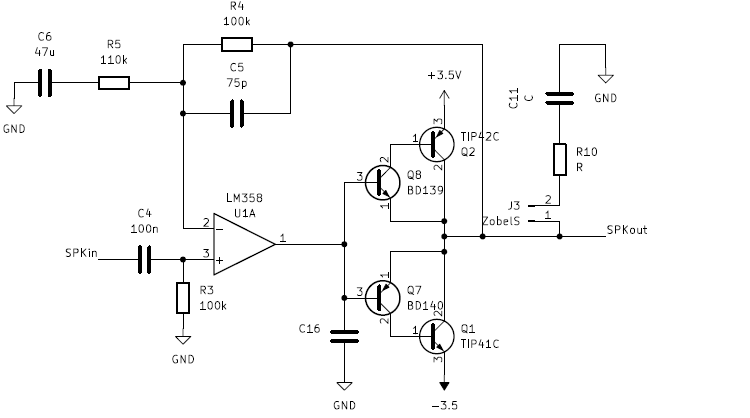
\includegraphics[width=0.7\textwidth]{images/2/2-2/circuitoAmplificadorAltavoces.png}
    \caption{Circuito amplificador de altavoces}
    \label{fig:2-2-amp-altavoz}
\end{figure}

\subsubsection{Diseño de PCB}

Todos estos sistemas se han integrado en una única PCB para intentar maximizar la integridad de la señal de audio, lo cual se consigue totalmente si se conecta el circuito sin tener en cuenta el \autoref{subsec:entre-dos-tierras}.

Hemos utilizado conectores Jack hembra de 3.5 mm para las dos entradas de audio y la salida a los auriculares. Un problema de este tipo de conectores es que el número de anillos puede variar en función de si los auriculares tienen o no micrófono y si son mono o estéreo. Si se quiere utilizar unos auricules con micrófono con nuestro sistema, se deben dejar ligeramente extraidos del conector para que haga mejor contacto la banda de tierra y mejorar significativamente el sonido.

La salida de altavoz se realiza a través de un terminal de dos tornillos para facilitar su conexión.

Como ya hemos comentado anteriormente, el circuito de transistores cuenta con un condensador de estabilizacion que finalmente no hemos utilizado. 

Además, hemos añadido la posibilidad de utilizar una red de Zobel, circuito que sirve para linealizar la respuesta en frecuencia de la inductancia intrínseca de los altavoces mediante un capacitor y una resistencia, pero finalmente no la hemos necesitado, por lo que tampoco está soldada.

El circuito cuenta además con un potenciómetro que sirve para ajustar el offset de la tensión de la tierra virtual gracias a los terminales específicos del \texttt{OP07}.

Hemos utilizado componentes SMT para los componentes pasivos y los conectores de audio y THT para los circuitos integrados, transistores y conectores de terminal.

Se puede ver una imagen del circuito finalizado en la \autoref{fig:2-2-circuito-foto} y el esquemático completo en el \autoref{anexo:circuito-audio}.

\begin{figure}[h]
    \centering
    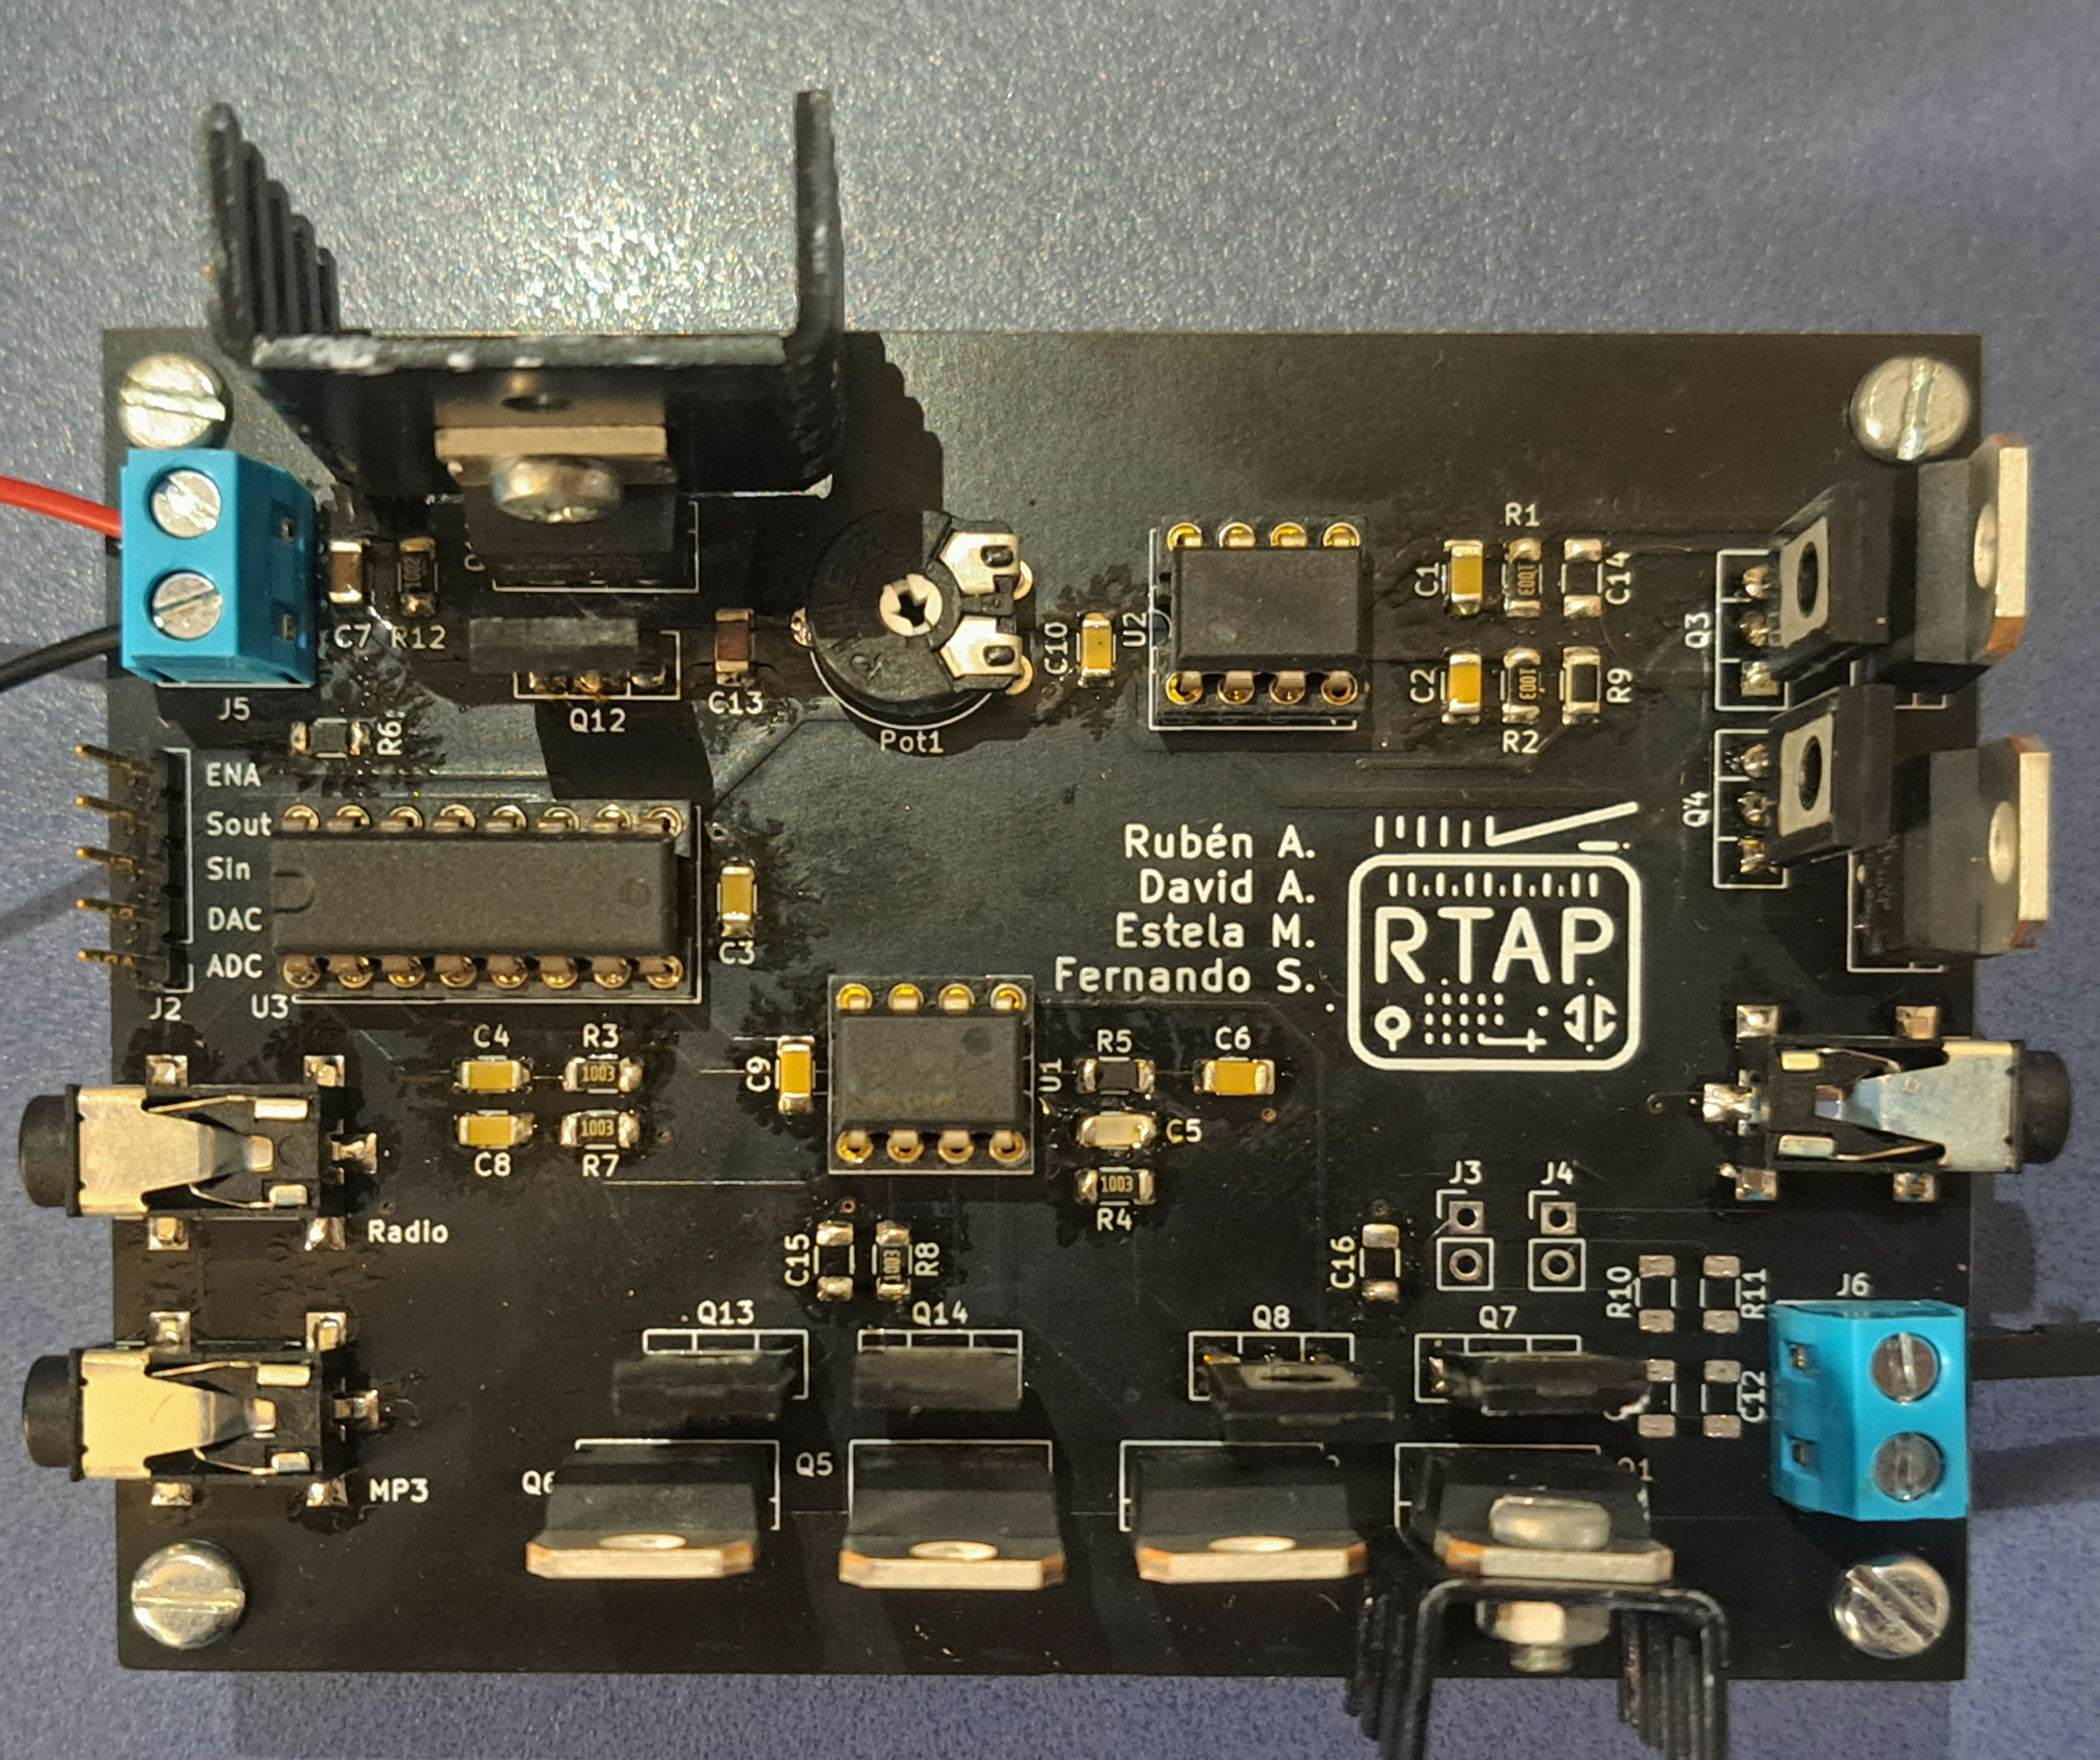
\includegraphics[width=0.5\textwidth]{images/2/2-2/circuito-foto.jpg}
    \caption{Circuito de audio completo}
    \label{fig:2-2-circuito-foto}
\end{figure}
\subsection{Módulo de radio}
El modelo de radio elegido ha sido el Sintonizador FM RDA5807M, mostrado en la \autoref{fig:2-3-Radio},  utilizado anteriormente en la asignatura de Sistemas Basados en Microprocesadores.

Dicho modelo se comunica con el microcontrolador mediante el protocolo \texttt{I2C}. El sintonizador cuenta con un decodificador MPX, salida de audio stereo y un rango de sintonización de 87 MHz a 108 MHz debido a nuestra situación geográfica.

En cuanto a la señal de audio de salida, hemos encontrado que presenta una componente continua de 1.65V y una amplitud de aproximadamente 1V. Debido a la conectividad que presenta el sintonizador, nos hemos encontrado el problema de que, al unirlo junto al resto del proyecto, cortocircuita la señal de masa analógica con la señal de masa virtual creada en nuestro circuito. Dicho problema se comentará en el \autoref{subsec:entre-dos-tierras}.

Por otra parte, necesita ser alimentado con una tensión entre 1.8V y 3.3V, soporta una corriente máxima de 10mA, cuenta con una relación señal-ruido típica de 55dB y presenta una distorsión armónica de audio total máxima del 0.2\%.

Todas las características de dicho sintonizador FM se han obtenido del datasheet ofrecido por el fabricante.
%REFERENCIA: DATASHEET RADIO

\begin{figure}[h]
    \centering
    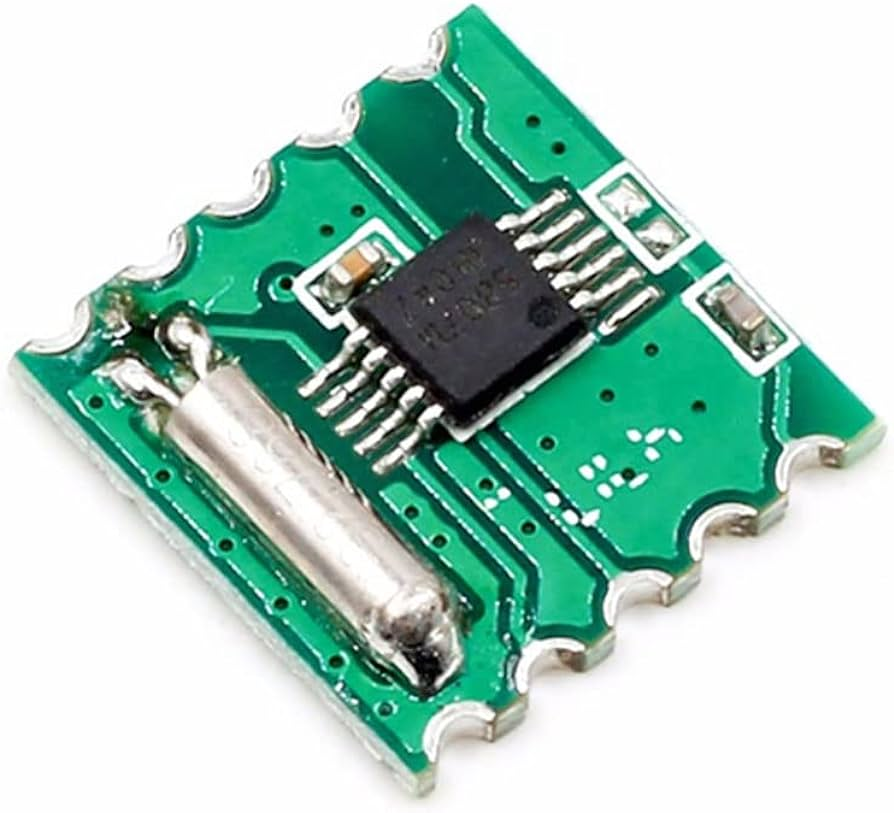
\includegraphics[width=0.3\textwidth]{images/2/2-3/Radio.jpg}
    \caption{Sintonizador FM RDA5807M}
    \label{fig:2-3-Radio}
\end{figure}
\subsection{Módulo MP3}
El modelo de MP3 seleccionado ha sido el YX5300, el cual se muestra en la \autoref{fig:2-3-MP3}.

Este reproductor se comunica con el microcontrolador mediante UART, con una velocidad de 9600 bps. También cuenta con una frecuencia de muestreo de 48 kHz y soporta tanto el formato MP3 como el formato WAV. Este modelo cuenta con un socket de tarjeta microSD en la cual se introducen las canciones, en los formatos antes mencionados, que se deseen reproducir. Dicha tarjeta deberá estar en formato Fat16 o Fat32 y tener como máximo \texttt{2 GB} de almacenamiento.

En cuento a la señal de audio obtenida a la salida del reproductor, podemos observar una salida bipolar entrada en 0V. Este comportamiento es totalmente inesperado ya que, al estar alimentado entre 3.3V y 0V, es extraño que la señal de salida pueda presentar valores negativos. Esto ha supuesto un gran problema en la unificación con el resto de módulos. Dicho problema y su solución será comentada en el \autoref{subsec:entre-dos-tierras}.

Por otra parte, el reproductor debe ser alimentadocon una tensión entre 3.2V y 5.2V, soporta una corriente máxima de 200mA y cuenta con un LED rojo que indica si está reproduciendo alguna canción.

Todas las características del reproductor MP3 se han obtenido del datasheet ofrecido por el fabricante. \cite{Catalex_MP3_boardPdf}

\begin{figure}[h]
    \centering
    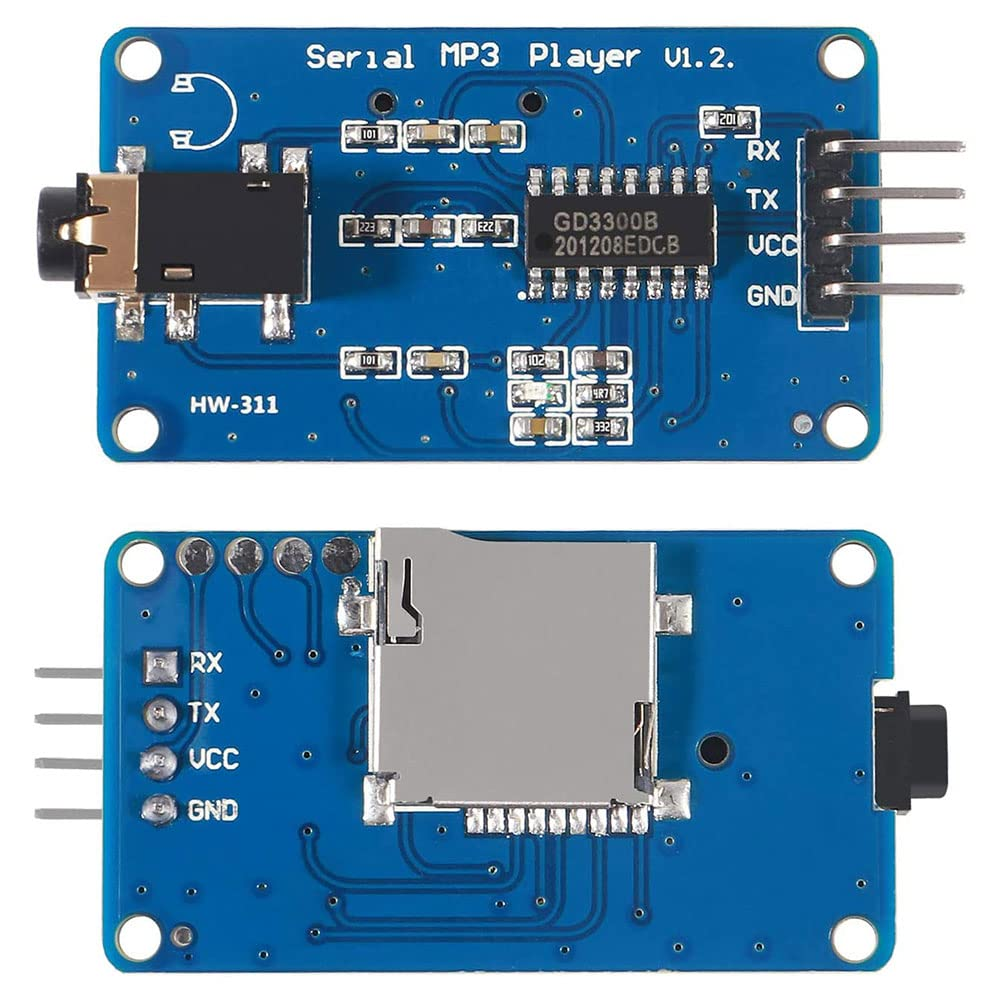
\includegraphics[width=0.3\textwidth]{images/2/2-4/MP3.jpg}
    \caption{Reproductor MP3 YX5300}
    \label{fig:2-3-MP3}
\end{figure}
\subsection{Módulo NFC}

Para su desarrollo, hemos utilizado el periférico I2C1, el protocolo RF, la placa \texttt{ANT7-T-M24SR64} \cite{M24SR64YPagWeb} de ST Microelectronics y la aplicación móvil \texttt{NFC Tools} \cite{NFCTools}. Además, a la hora de realizar comprobaciones desarrollando el módulo, hemos utilizado la app \texttt{ST25} \cite{ST25}.

\texttt{ANT7-T-M24SR64}: 
La placa \texttt{ANT7-T-M24SR64} es una placa que incluye un \texttt{M24SR64-Y}. \texttt{M24SR64-Y} es una tag dinámica NFC/RFID, EEPROM de interfaz dual, con protocolos RF e I2C. Se puede operar desde una interfaz I2C, un lector RFID o un teléfono con NFC.

\begin{figure}[h]
    \centering
    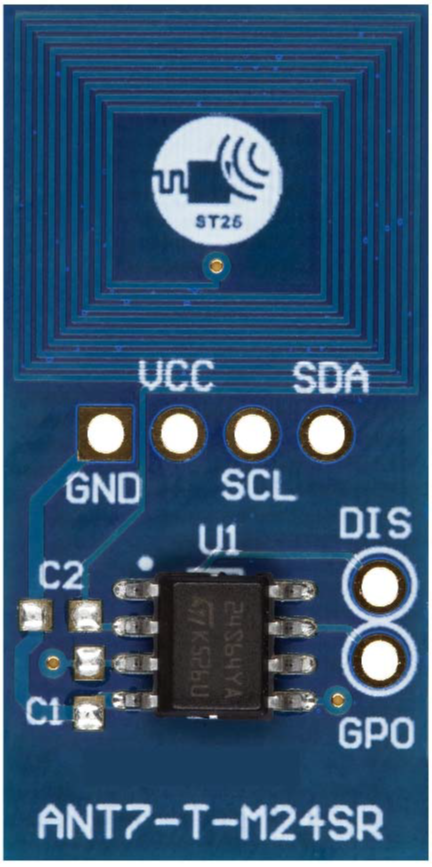
\includegraphics[width=0.15\textwidth]{images/2/2-5/M24SR.png}
    \caption{Módulo NFC \texttt{ANT7-T-M24SR64}}
    \label{fig:2-5-modulo-nfc}
\end{figure}

Como se puede observar en la figura anterior, hay 6 pines:

\begin{itemize}
    \item \texttt{VCC}: Alimentación 3.3 V.
    \item \texttt{GND}: Masa.
    \item \texttt{SDA}: Línea de datos del bus I2C.
    \item \texttt{SCL}: Señal de reloj del bus I2C.
    \item \texttt{GPO}: A nivel bajo, RF o I2C está siendo utilizado. A nivel alto, está libre.
    \item \texttt{DIS}: Activación/Desactivación de los comandos RF.
\end{itemize}

\subsection{Entre Dos Tierras}
\label{subsec:entre-dos-tierras}

El mayor problema al que nos hemos enfrentado en este proyecto es la gestión de las tierras en las señales de audio. Inicialmente diseñamos el circuito para que las señales de audio se conectaran entre la entrada de audio y la tierra virtual del circuito analógico, pensando que las señales serían compatibles con la entrada del ADC al estar alimentadas con los mismos niveles de tensión que los que las generan.

Sin embargo, descubrimos posteriormente que los circuitos compartían la tierra de audio de la entrada directamente con la salida, por lo que se realizaba un cortocircuito directo entre la tierra de la alimentación (o alimentación negativa visto desde el amplificador de audio) y la tierra virtual, por lo que se cortocircuitaban 3.5 V. 

Esto era claro en el lado del MP3 ya que el cortocircuito era a través de un camino de baja impedancia y provocaba que se activara la protección, desactivando la salida de audio. Sin embargo, debido a la circuitería interna o a las conexiones de la radio, había una pequeña pero no mínima impedancia que provocaba un consumo muy elevado de corriente pero que no llegaba al amperio, por lo que la protección no se disparaba. Esto es muy peligroso ya que es una potencia que se está disipando en el interior del chip y probablemente provoque daños si se mantiene el circuito en dicha condición.

Para solucionar este problema, decidimos construir unos cables de sonido en los cuales solo se conecte el terminal que lleva la señal, deshaciendo la conexión que realizan los sensores internamente.

Con estos ajustes la radio funcionaba bien, sin demasiado problema (excepto el ruido del que hablaremos a continuación). Sin embargo, el MP3 presenta otro problema. Contraintuitivamente, a pesar de estar alimentado con una tensión unipolar, el circuito del MP3 consigue generar una tensión bipolar simétrica con la señal de audio, señal completamente incompatible con nuestro sistema de muestreo con un ADC de la placa.

Para mediar este problema, hemos montado otro circuito analógico accesorio que mediante un divisor de tensión simétrico y un condensador de desacoplo consigue añadir una componente continua de 1.65 V a la tensión simétrica de entrada, haciendola completamente compatible con el sistema. Se añade una resistencia de \textit{Pull-down} en la entrada para evitar picos de tensión en el encendido del sistema. Los valores de las resistencias pueden ser cualesquiera valores grandes siempre que sean iguales y el condensador interesa elegirlo lo más grande posible. El circuito está recogido en la \autoref{fig:2-6-sumador}. 

\begin{figure}[h]
    \centering
    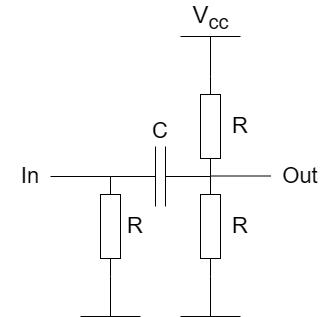
\includegraphics[width=0.5\textwidth]{images/2/2-6/sumadorEsquematico.png}
    \caption{Esquemático del circuito sumador}
    \label{fig:2-6-sumador}
\end{figure}

Se ha montado el circuito sobre una placa de baquelita, como se puede ver en la imagen de la \autoref{fig:2-6-foto-sumador}.\ 

\begin{figure}[h]
    \centering
    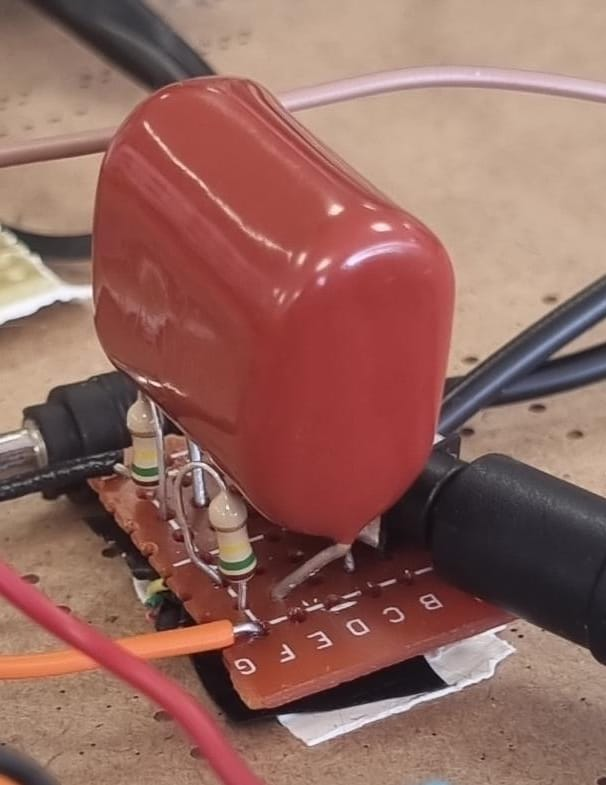
\includegraphics[width=0.25\textwidth]{images/2/2-6/fotoSumador.jpg}
    \caption{Foto del circuito sumador analógico}
    \label{fig:2-6-foto-sumador}
\end{figure}

Hemos elegido un valor de $100\ k\Omega$ para las resistencias y aproximadamente $1\ \mu F$ para el condensador, lo cual nos ofrece buenos resultados. Sin embargo, primero realizamos las pruebas con un condensador cerámico y no conseguimos que la tensión se estabilizara, por lo que se desplazaba el valor lentamente hacia uno de los raíles de alimentación. La solución que encontramos fue sustituirlo por un condensador de tántalo, que si bien tiene un tamaño físico considerablemente superior, consigue mantener de manera muy estable la tensión del circuito.

Este circuito funciona correctamente pero tiene la desventaja de decrementar ligeramente la tensión de entrada, provocando una caída en la relación señal-ruido del sistema.

Una vez solucionado el problema de las masas, aparece un ruido muy elevado en forma de zumbido y ruido blanco, por lo que el audio es de bastante baja relacion calidad ruido. Esto es principalmente debido a la longitud de los conductores por lo que va la señal, la cantidad de circuitos que atraviesa, etcétera. 

Además, la desconexión de las masas de los cables de audio provoca que el camino de retorno de las señales tenga que atravesar el resto del circuito y se deja de tratar la señal como un par diferencial, por lo que se pierde bastante calidad debido a la diferencia de tensión en las masas y algún posible bucle de masa al que se le acople algún ruido.

Por todo ello, si se quiere disfrutar de la máxima calidad de audio que puede ofrecer nuestro circuito, se debe desconectar la masa de la placa de la del circuito de amplificación de audio. El principal inconveniente de ello es que se deja de poder gestionar el multiplexor y la habilitación a través de los GPIO y no se puede realizar el procesado digital de señales.

Si se conectan los pines de selección y habilitación a los raíles de alimentación para seleccionar la configuración y se conecta un jumper entre los pines de ADC y DAC, se tiene una buenísima calidad de sonido, tanto en el altavoz como en los cascos. Se puede igualmente controlar la radio y el MP3 mediante las interfaces ya que eso no depende de la masa del circuito.

La mejor solución a este problema sería la realización de un circuito con alimentación simétrica verdadera. Esto se podría conseguir mediante dos baterías en serie (aunque sería un desperdicio ya que una solo se utilizaría para la parte negativa de la señal y no alimentaría la placa) o mediante la generación de una tensión negativa con un convertidor, por ejemplo, de tipo reductor-elevador con topología inversora. Igualmente se tendría que tener en cuenta la naturaleza bipolar de la señal del MP3 y se debería incluir el circuito de \textit{offset} a la placa o utilizar un cambiador de nivel analógico.
\subsection{Conexión de la alimentación a la placa}

Otro problema significativo que hemos encontrado es la conexión de la placa a la alimentación por baterías. La placa \texttt{STM32F769NI-Disco} indica que se puede alimentar con una tensión de entre 7 y 12 voltios en el pin de \texttt{Vin} siempre que se seleccione \texttt{ext5V} en los jumpers de selección de alimentación.

Probamos a alimentarlo con una fuente de tensión de laboratorio y el circuito funcionaba adecuadamente, consumiendo aproximadamente $300\ mA$. Sin embargo, al alimentarlo desde nuestro subsistema analógico, la placa funciona adecuadamente durante aproximadamente cinco segundos para después quedarse congelado. Hemos podido comprobar que es únicamente la CPU que se congela ya que las DMAs de audio siguen funcionando, reproduciendo el último contenido del buffer en bucle.

Hemos comprobado que no es un problema de tensión ya que, aunque en la hoja de catálogo indique que la placa requiere de mínimo 7 voltios, funciona bien incluso con $6.5\ V$ de la fuente de alimentación.

Tampoco es un problema de corriente ya que, como se explica en el apartado de test hardware, la placa puede aportar mucha más corriente que el aproximadamente medio amperio que requiere la placa.
